\chapter{Inference in Dynamical Systems}
\label{c:inferenceInDynamicalSystems}



Out second contribution is to take a probabilistic perspective on "classical" Koopman theory as presented in various publications~\cite{bruntonKoopmanInvariantSubspaces2016,hanDeepLearningKoopman2020,kaiserDatadrivenDiscoveryKoopman2020,luschDeepLearningUniversal2018,williamsDataDrivenApproximation2015}. In this chapter we will build the groundwork for variational inference to combine them to the single \algname algorithm presented in~\autoref{c:nonlinearGaussianKoopman}.

\section{Hidden Markov Models and LGDS}
	\acp{hmm} are simple Bayesian networks described by a non-observable (\emph{hidden}) Markov chain. This non-observable discrete chain can be indirectly observed with measurements that are emitted by every state. One of the key features of a Markov chain is that a state does only depend on the previous state, but not on the second previous, third previous, and so on, states. That is, knowing only the previous state is sufficient and no more information can be gathered by knowing every other state before. This is described by the state transition distribution
	\begin{equation*}
		s_{k + 1} \sim p(s_{k + 1} \given s_k)
	\end{equation*}
	being only dependent on the previous state \(s_k\). Analogous, a measurement \(\vec{y}_k\) of a state \(s_k\) is only dependent on that specific state:
	\begin{equation*}
		\vec{y}_k \sim p(\vec{y}_k \given s_k)
	\end{equation*}
	These assumptions are called the \emph{Markov property} and a system fulfilling this property is called \emph{Markovian}. These conditional distributions can be written in a graphical model as shown in~\autoref{fig:hiddenMarkovModel}. Note that, in general, no assumption has to be made on the "type" of state/observation (\ac{ie} whether it is a scalar, a vector or something completely different). Also, no assumption is made on the specific transition distributions, \acp{hmm} can also be used to model deterministic transitions using a Dirac delta distribution.

	\begin{figure}
		\centering
		\tikzHiddenMarkovModel
		\caption{Illustration of a completely general Hidden Markov Model with states \(s_k\) and emissions/observations \(\vec{y}_k\).}
		\label{fig:hiddenMarkovModel}
	\end{figure}

	A set of closely related dynamics models are \acp{lgds} which are described by a noisy state transition
	\begin{equation*}
		\vec{s}_{t + 1} = \mat{A} \vec{s}_t + \vec{w}_t,\quad \vec{w}_t \sim \normal(\vec{0}, \mat{Q})
	\end{equation*}
	with covariance matrix \(\mat{Q}\). Similarly, the measurements \( \vec{y}_t = \mat{C} \vec{s}_t + \vec{v}_t \) underlie a Gaussian noise \( \vec{v}_t \sim \normal(\vec{0}, \mat{R}) \) too. Together they form the probabilistic model
	\begin{align*}
		\vec{s}_{t + 1} &= p(\mat{A} \vec{s}_t, \vec{Q}) \\
		\vec{y}_t &= p(\mat{C} \vec{s}_t, \mat{R})
	\end{align*}
	which fulfills the Markov property, hence the system is Markovian:
	\begin{equation*}
		p(\vec{s}_{1:T}, \vec{y}_{1:T}) = p(\vec{s}_1) \prod_{t = 2}^{T} p(\vec{s}_t \given \vec{s}_{t - 1}) \prod_{t = 1}^{T} p(\vec{y}_t \given \vec{s}_t)
	\end{equation*}
	Note that we write \( \vec{s}_{t_0:t_1} \) for the sequence \( \big( \vec{s}_{t_0}, \vec{s}_{t_0 + 1}, \cdots, \vec{s}_{t_1} \big) \) and analogous for the observation sequence \( \vec{y}_{t_0:t_1} \). The probabilistic model of a \ac{lgds} is shown in~\autoref{fig:lgds}.

	This system is similar to a \ac{hmm} and in fact a \ac{lgds} really is an \ac{hmm}, just with continuous states \( \vec{s}_t \in \R^k \) and measurements \( \vec{y}_t \in \R^p \).

	\begin{figure}
		\centering
		\tikzLinearGaussianDynamicalSystem
		\caption{Illustration of a Linear Gaussian Dynamical System with states \(\vec{x}_t\) and observations \(\vec{y}_t\). Solid arrows represent probabilistic dependency, where the matrix \(\mat{A}\) is the dynamics matrix indicating that the mean transitions linearly, so do the observations with the observation matrix \(\mat{C}\).}
		\label{fig:lgds}
	\end{figure}
% end

\section{Inference: Filtering and Smoothing}
	When looking at an \ac{lgds}, one of the first problems that one might consider is how to get the states (also called \emph{latent states} as we cannot observe) them back? This procedure is called \emph{inference}. In this section we will give an overview on how to perform inference on an \ac{lgds}, so on a linear system that behaves Markovian.

	For time-series data, the inference procedure is widely know as \emph{filtering} ans \emph{smoothing}, where the following distributions on the latent states \( \vec{s}_t \) are calculated:
	\begin{itemize}
		\item Filtering: \tabto{2.5cm} \( p(\vec{s}_t \given \vec{y}_{1:t}) \)
		\item Smoothing: \tabto{2.5cm} \( p(\vec{s}_t \given \vec{y}_{1:T}) \)
	\end{itemize}
	That is, the filtered distribution only depends on the measurements \emph{to that time} where in contrast the smoothed distribution has used all data to the last time step \(T\) to estimate the latent states. An intermediate step in the filtering algorithm is called \emph{prediction} where the distribution \( p(\vec{s}_t \given \vec{y}_{1:t - 1}) \) is being calculated, using only the data to the previous time step. The differences between what data is used in the three steps is shown in~\autoref{fig:predictionFilteringSmoothing}.

	We will now take a look on the most used filter, the well-known \emph{Kalman Filter} and its colleague, the \emph{Rauch-Tung-Striebel Smoother}, which is also sometimes called the \emph{Kalman Smoother} as it requires a run of the Kalman filter first.

	\begin{figure}
		\centering
		\tikzPredictionFilteringSmoothing
		\caption{This diagram shows the main differences between prediction, filtering and smoothing. The shaded region describes the measurements that has been used to estimate the state at time step \(t\), indicated by a solid line. The dotted line represents time step \(t - 1\), to which all measurements are used in all three procedures. \\ Adopted from~\cite{solinCubatureIntegrationMethods2010}.}
		\label{fig:predictionFilteringSmoothing}
	\end{figure}

	\subsection{Kalman Filter}
		The Kalman filter as originally introduced by R.~Kalman in 1960~\cite{kalmanNewApproachLinear1960} in the context of signal processing to predict random signals, separate them signals from noise and detect signals of known form in the presence of noise~\cite{kalmanNewApproachLinear1960}. The normal Kalman filter assumes an underlying model of the form of an \ac{lgds} where the measurements are detected and the state is to be estimated from the data. The process of estimated the states is done in a two-step fashion:
		\begin{enumerate}
			\item Prediction: \tabto{2.5cm} Estimate the distribution \( p(\vec{s}_t \given \vec{y}_{1:t - 1}) \)
			\item Correction: \tabto{2.5cm} Estimate the distribution \( p(\vec{s}_t \given \vec{y}_{1:t}) \)
		\end{enumerate}
		For a simple linear system with Gaussian noise, \ac{ie} an \ac{lgds}, the equations for both the prediction and the correction can be given in closed form and are fairly straightforward. For the prediction step, the equations are given as
		\begin{align*}
			\vec{s}_{t \subgiven t - 1} &= \mat{A} \vec{s}_{t - 1 \subgiven t - 1} \\
			\mat{P}_{t \subgiven t - 1} &= \mat{A} \mat{P}_{t - 1 \subgiven t - 1} \mat{A}^T + \mat{Q}
		\end{align*}
		where \( \vec{s}_{t \given t - 1} \) and \( \mat{P}_{t \given t - 1} \) are the mean and covariance of the prediction distribution \( p(\vec{s}_t \given \vec{y}_{1:t - 1}) \), respectively. The correction step, which integrated new knowledge gained from the observation \( \vec{y}_t \) into the estimated, is given as
		\begin{align*}
			\vec{s}_{t \subgiven t} &= \vec{s}_{t \subgiven t - 1} + \mat{K}_t \vec{y}_{t \subgiven t - 1} \\
			\mat{P}_{t \subgiven t} &= \mat{P}_{t \subgiven t - 1} - \mat{K}_t \mat{S}_t \mat{K}_t^T
		\end{align*}
		with the auxiliary variables
		\begin{align*}
			\vec{y}_{t \subgiven t - 1} &= \vec{y}_t - \mat{C} \vec{s}_{t \subgiven t - 1} \\
			\mat{S}_t &= \mat{C} \mat{P}_{t \subgiven t - 1} \mat{C}^T + \mat{R} \\
			\mat{K}_t &= \mat{P}_{t \subgiven t - 1} \mat{C}^T \mat{S}_t^{-1}
		\end{align*}
		known as the innovation, residual covariance and Kalman gain. The resulting estimates \( \vec{s}_{t \subgiven t} \) and \( \mat{P}_{t \subgiven t} \) then form the mean and covariance of the filtered distribution \( p(\vec{s}_t \given \vec{y}_{1:t}) \), respectively. These equations form a recursive algorithm "forward in time" starting off with initial state estimates \( \vec{s}_{0 \subgiven 0} = \vec{m}_0 \) and \( \mat{P}_{0 \subgiven 0} = \mat{V}_0 \) that have to be determined in another way.

		But these equations only work for linear systems. Lots of extensions of the regular Kalman filter have been proposed to extend the filter to nonlinear systems. The most used one is the \ac{ekf} which assumes locally linear dynamics and uses first-order Taylor expansions to linearize them. Throughout this thesis we will use the cubature Kalman filter, which we will introduce later in~\autoref{sec:cubatureFiltering}.
	% end

	\subsection{Rauch-Tung-Striebel/Kalman Smoother}
		The \ac{rts} smoother has been introduced five years after the original Kalman filter in the 1965 by H.~E.~Rauch, F.~Tung and C.~T.~Striebel~\cite{rauchMaximumLikelihoodEstimates1965} exhibiting the equations for optimal smoothing of linear systems with Gaussian noise, \ac{ie} \ac{lgds}. With the smoother, we want to estimate the smoothed distribution, also called the \emph{posterior}
		\begin{equation*}
			p(\vec{s}_t \given \vec{y}_{1:T})
		\end{equation*}
		which uses all measurements (see again~\autoref{fig:predictionFilteringSmoothing} for an illustration). With letting the Kalman filter "run" beforehand, we have the filtered distribution \( p(\vec{s}_t \given \vec{y}_{1:t}) \) at hand. Then we have the smoothing equations as
		\begin{align*}
			\vec{s}_{t \subgiven T} &= \vec{s}_{t \subgiven t} + \mat{J}_t (\vec{s}_{t + 1 \subgiven T} - \vec{s}_{t + 1 \subgiven t}) \\
			\mat{P}_{t \subgiven T} &= \mat{P}_{t \subgiven t} + \mat{J}_t (\mat{P}_{t + 1 \subgiven T} - \mat{P}_{t + 1 \subgiven t}) \mat{J}_t^T
		\end{align*}
		with the auxiliary variable \( \mat{J}_t = \mat{P}_{t \subgiven t} \mat{A}^T \mat{P}_{t + 1 \subgiven t}^{-1} \). The resulting estimates \( \vec{s}_{t \subgiven T} \) and \( \mat{P}_{t \subgiven T} \) then form the mean and covariance of the smoothed/posterior distribution \( p(\vec{s}_t \given \vec{y}_{1:T}) \). These equations form a recursive algorithm "backward in time" starting off with the final state and covariance estimates of the filter.

		Hence, we need the Kalman filter before using the \ac{rts} smoother. Due to this hard wiring between the two algorithms, the \ac{rts} smoother is also often referred to as the Kalman smoother.

		Note that these equations only depend on the state dynamics matrix \( \mat{A} \), so a system that is linear in the state and nonlinear in the measurements can still use the standard \ac{rts} smoother and no further modification is required.
	% end
% end

\section{Cubature Rules and Filtering}
	\label{sec:cubatureFiltering}

	As we have already discussed is the plain Kalman filter not applicable to nonlinear systems without modifications. In this section we want to motivate the need for \emph{cubature rules} and outline their derivation and how to apply them.

	Often when deriving probabilistic algorithms like \ac{em} or the Kalman filter, we face us to evaluate expectations \( \E_{\vec{x} \sim p(\vec{x})}\big[ \vec{f}(\vec{x}) \big] \) and hence integrals of the form
	\begin{equation*}
		\E_{\vec{x} \sim p(\vec{x})}\big[ \vec{f}(\vec{x}) \big] = \int\! \vec{f}(\vec{x}) p(\vec{x}) \dd{\vec{x}}
	\end{equation*}
	In this thesis and lots of other literature, we experience Gaussian distributions \( p(\vec{x}) = \normal(\vec{x} \given \vec{\mu}, \mat{\Sigma}) \) with mean \(\vec{\mu}\) and covariance \(\mat{\Sigma}\), leading to Gaussian integrals of the form
	\begin{equation*}
		\E_{\vec{x} \sim p(\vec{x})}\big[ \vec{f}(\vec{x}) \big] = \int\! \vec{f}(\vec{x}) \, \normal(\vec{x} \given \vec{\mu}, \mat{\Sigma}) \dd{\vec{x}}
	\end{equation*}
	which do not have closed form solutions for arbitrary, nonlinear, functions \( \vec{f}(\vec{x}) \). Two common approaches for approximating the expectations/integrals are Monte Carlo Estimation, leading to particle filters, and numerical integration methods, known as quadrature/cubature\footnote{As we are integrating in multiple dimensions at once, the name "cubature" makes more sense than "quadrature".} rules.

	To approximate Gaussian integrals, we need a set of \(m\) points \( \vec{x}_i \) to evaluate \( \vec{f}(\vec{x}) \) at and a set weights \( w_i \) to form a sum over the points:
	\begin{equation*}
		\int\! \vec{f}(\vec{x}) \, \normal(\vec{x} \given \vec{\mu}, \mat{\Sigma}) \dd{\vec{x}} \approx \sum_{i = 1}^{m} w_i \vec{f}(\vec{x}_i)
	\end{equation*}
	In this thesis we utilize the spherical-radial cubature rule~\cite{solinCubatureIntegrationMethods2010} which is a third-degree approximation for Gaussian integrals. A third-degree approximation means that "this rule exact for all monomials up to degree three"~\cite[p. 18]{solinCubatureIntegrationMethods2010}. In this cubature rule, the approximation a finite sum over \( 2n \) points, where \( n \) is the dimensionality of \(\vec{x}\), \ac{ie} \( \vec{x} \in \R^n \). With \( \sqrt{\mat{\Sigma}} \) being the Cholesky decomposition of \( \mat{\Sigma} \), so \( \mat{\Sigma} = \sqrt{\mat{\Sigma}} \sqrt{\mat{\Sigma}}^T \), the approximation is given as
	\begin{equation*}
		\int\! \vec{f}(\vec{x}) \, \normal(\vec{x} \given \vec{\mu}, \mat{\Sigma}) \dd{\vec{x}} \approx \frac{1}{2N} \sum_{i = 1}^{2n} \vec{f}(\sqrt{\mat{\Sigma}} \vec{\xi}_i - \vec{\mu})
	\end{equation*}
	with the cubature points \( \vec{\xi}_i = \sqrt{n} [\vec{1}]_i \). Here the points \( [\vec{1}]_i \) are "from the intersections between the Cartesian axes and the \(n\)-dimensional unit hypersphere"~\cite{solinCubatureIntegrationMethods2010}. That is, the point \( [\vec{1}]_i \) is the \(i\)-th row vector of the block matrix \( \begin{bmatrix} \mat{I} & -\mat{I} \end{bmatrix} \), where \( \mat{I} \) is the \(n\)-dimensional identity matrix.

	\autoref{fig:cubature} shows the spherical-radial cubature rule working on a transition from polar coordinates to Cartesian coordinates where the transformation is given by:
	\begin{equation*}
		x = r \cos\theta \qquad\qquad y = r \sin\theta
	\end{equation*}
	The polar coordinate particles have been sampled from a multivariate Gaussian with diagonal covariance:
	\begin{equation*}
		r \sim \normal(80,\, 40) \qquad\qquad \theta \sim \normal(40,\, 0.4)
	\end{equation*}

	\begin{figure}
		\centering
		\begin{subfigure}[t]{0.5\linewidth}
			\centering
			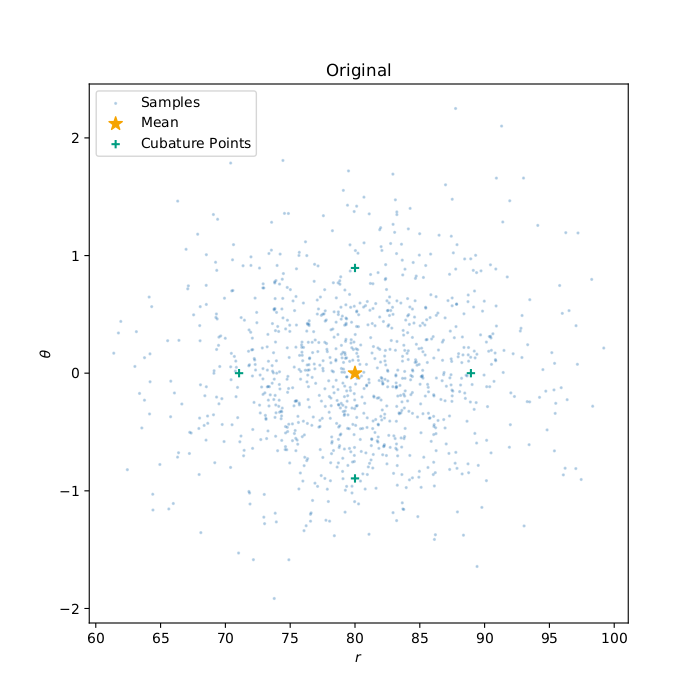
\includegraphics[width = \linewidth]{figures/inference/cubature/spherical-radial-cubature-original}
			\caption{The original samples in polar coordinates with the real mean shown as an orange star in the middle. The cubature points are shown as green crosses.}
		\end{subfigure}%
		~
		\begin{subfigure}[t]{0.5\linewidth}
			\centering
			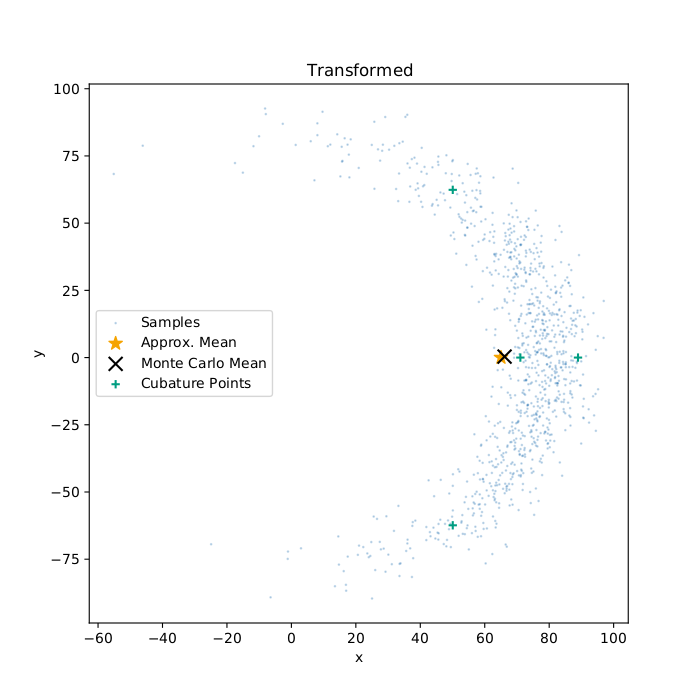
\includegraphics[width = \linewidth]{figures/inference/cubature/spherical-radial-cubature-transformed}
			\caption{The approximate mean calculated via the spherical-radial cubature rule is shown as an orange star, positioned at the mean of the transformed cubature points (red crosses). This plot also shows the Monte Carlo  as a green cross right above the cubature estimate, showing that the cubature estimate is really accurate with significantly less computational effort.}
		\end{subfigure}
		\caption{These plots show how the spherical-radial cubature rule is used to estimate the mean of the Gaussian on the left after it has been transformed with a polar transformation to the right. To illustrate the shape of the Gaussian after it has been transformed, we added the blue dots as sample values of the Gaussian. These are 1000 sample points also used to calculate the Monte Carlo estimate of the mean.}
		\label{fig:cubature}
	\end{figure}

	\subsection{Square-Root Filtering/Smoothing}
		\todo{Cubature: Sqrt Filtering}
	% end
% end
